% Created 2015-06-14 Dom 22:16
\documentclass[11pt]{article}
\usepackage[utf8]{inputenc}
\usepackage[T1]{fontenc}
\usepackage{fixltx2e}
\usepackage{graphicx}
\usepackage{longtable}
\usepackage{float}
\usepackage{wrapfig}
\usepackage{rotating}
\usepackage[normalem]{ulem}
\usepackage{amsmath}
\usepackage{textcomp}
\usepackage{marvosym}
\usepackage{wasysym}
\usepackage{amssymb}
\usepackage{hyperref}
\tolerance=1000
\usepackage{minted}
\usemintedstyle{perldoc}
\usepackage{tikz}
\usetikzlibrary{decorations.markings}
\tikzstyle{vertex}=[circle, draw, inner sep=0pt, minimum size=7pt]
\newcommand{\vertex}{\node[vertex]}
\author{Alice Duarte Scarpa, Bruno Lucian Costa}
\date{2015-06-23}
\title{Trabalho de Estrutura de Dados e Algoritmos}
\hypersetup{
  pdfkeywords={},
  pdfsubject={},
  pdfcreator={Emacs 24.4.1 (Org mode 8.2.10)}}
\begin{document}

\maketitle

\section{Exercício 6.30 (Papadimitriou)}
\label{sec-1}
\subsection{Enunciado}
\label{sec-1-1}

\textit{Reconstruindo árvores filogenéticas pelo método da máxima parcimônia}

Uma árvore filogenética é uma árvore em que as folhas são espécies
diferentes, cuja raiz é o ancestral comum de tais espécies e cujos
galhos representam eventos de especiação.

Queremos achar:

\begin{itemize}
\item Uma árvore (binária) evolucionária com as espécies dadas
\item Para cada nó interno uma string de comprimento $k$ com a
sequência genética daquele ancestral.
\end{itemize}


Dada uma árvore acompanhada de uma string $s(u) \in \{A, C, G, T\}^k$ para
cada nó $u \in V(T)$, podemos atribuir uma nota usando o método da
máxima parcimônia, que diz que menos mutações são mais prováveis:
\[ \mathrm{nota}(T) = \sum_{(u,v) \in E(T)} (\text{número de posições em que }s(u)\text{ e }s(v)\text{ diferem}). \]

Achar a árvore com nota mais baixa é um problema difícil. Aqui vamos
considerar um problema menor: Dada a estrutura da árvore, achar as
sequências genéticas $s(u)$ para os nós internos que dêem a nota mais
baixa.

Um exemplo com $k = 4$ e $n = 5$:

\href{http:github.com/adusca/FGV-EDA/6_30/tree.png}{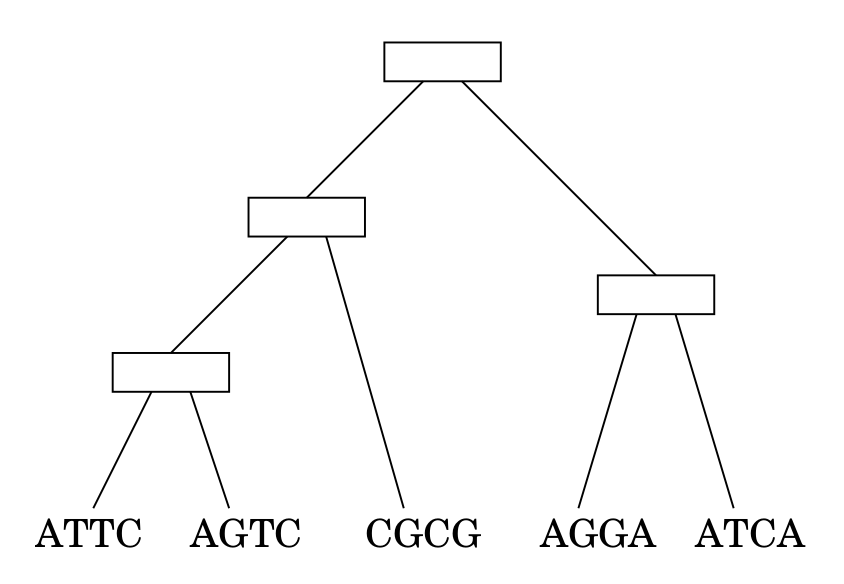
\includegraphics[width=.9\linewidth]{6_30/tree.png}}

\begin{enumerate}
\item Ache uma reconstrução para o exemplo seguindo o método da
máxima parcimônia.
\item Dê um algoritmo eficiente para essa tarefa.
\end{enumerate}


\subsection{Dados reais}
\label{sec-1-2}

Usamos \url{http://www.ncbi.nlm.nih.gov/Taxonomy/CommonTree/wwwcmt.cgi} para gerar o banco de dados.

Rosalind MULT, GLOB, EDTA, PERM, EDIT, LCSQ,
CSTR, CTBL, NWCK, SSET, MRNA, KMP, PROB
SSEQ, SPLC, LCSM


\section{Exercício 6.3 (Papadimitriou)}
\label{sec-2}

\subsection{Enunciado}
\label{sec-2-1}

O Yuckdonald's está considerando abrir uma cadeia de restaurantes em
Quaint Valley Highway (QVG). Os $n$ locais possíveis estão em uma
linha reta, e as distâncias desses locais até o começo da QVG são, em
milhas e em ordem crescente, $m_1, m_2, \ldots, m_n$. As restrições
são as seguintes:

\begin{itemize}
\item Em cada local, o Yuckdonald's pode abrir no máximo um
restaurante. O lucro esperado ao abrir um restaurante no local
$i$ é $p_i$, onde $p_i > 0$ e $i = 1, 2, \ldots, n$.
\item Quaisquer dois restaurantes devem estar a pelo menos $k$
  milhas de distância, onde $k$ é um inteiro positivo.
\end{itemize}

Dê um algoritmo eficiente para computar o maior lucro total
esperado, sujeito às restrições acima.




\section{Exercício 7.28 (Tardos)}
\label{sec-3}

\subsection{Enunciado}
\label{sec-3-1}

Um grupo de estudantes está escrevendo um módulo para preparar
cronogramas de monitoria. O protótipo inicial deles funciona do
seguinte modo: O cronograma é semanal, de modo que podemos nos focar
em uma única semana.

\begin{itemize}
\item O administrador do curso escolhe um conjunto de $k$
intervalos disjuntos de uma hora de duração $I_1, I_2, \ldots,
      I_k$, nos quais seria possível que monitores dessem suas
monitorias; o cronograma final consistirá de um subconjunto de
alguns (mas geralmente não todos) esses intervalos.
\item Cada monitor então entra com seu horário semanal, informando
as horas em que ele está disponível para monitorias.
\item O administrador então especifica, para parâmetros $a$, $b$ e
$c$, que cada monitor deve dar entre $a$ e $b$ horas de
monitoria por semana, e que um total de $c$ horas de monitoria
deve ser dado semanalmente.
\end{itemize}

O problema é escolher um subconjunto dos horários (intervalos) e
atribuir um monitor a cada um desses horários, respeitando a
disponibilidade dos monitores e as restrições impostas pelo
administrador.


a) Dê um algoritmo polinomial que ou constrói um cronograma
   válido de horas de monitoria (especificando que monitor cobre
   quais horários) ou informa que não há cronograma válido.


b) O algoritmo acima tornou-se popular, e surgiu a vontade de
   controlar também a densidade das monitorias: dado números $d_i$,
   com $i$ entre $1$ e $5$, queremos um cronograma com pelo menos
   $d_i$ horários de monitoria no dia da semana $i$. Dê um
   algoritmo polinomial para resolver o problema com essa restrição
   adicional.

\subsection{Solução força-bruta}
\label{sec-3-2}

\subsubsection{Algoritmo}
\label{sec-3-2-1}

\subsubsection{Implementação}
\label{sec-3-2-2}

\subsubsection{Complexidade}
\label{sec-3-2-3}
\subsection{Solução usando fluxo}
\label{sec-3-3}

\subsubsection{Introdução}
\label{sec-3-3-1}

Queremos modelar esse problema como um problema de fluxo. Para isso
vamos começar com algumas definições de fluxo.

\begin{enumerate}
\item Definições
\label{sec-3-3-1-1}

Uma rede de fluxo é um grafo direcionado $G =
(V, E)$ com as seguintes propriedades:
\begin{itemize}
\item Existe um único vértice \textit{fonte} $s \in V$. Nenhuma aresta entra em $s$.
\item A cada aresta $e$ está associada uma capacidade inteira $c_e$ e
uma demanda $d_e$ tal que $c_e \geq d_e \geq 0$.
\item Existe um único vértice \textit{dreno} $t \in V$. Nenhuma aresta sai de $t$.
\end{itemize}

Um fluxo $f$ de $s$ a $t$ é uma função $f \colon E \to R^+$ que associa a cada
aresta $e$ um valor real não-negativo $f(e)$ tal que:

\begin{enumerate}
\item $\forall e \in E, d_e \leq f(e) \leq c_e$
\item Para todo nó $v \not\in \{s,t\}$:
\[ \sum_{e \text{ chegando em } v} f(e) = \sum_{e \text{ saindo de } v} f(e) \]
\end{enumerate}

$f(e)$ representa o fluxo que vai passar pela aresta $e$. O valor de
um fluxo é o total que parte da fonte $s$, isso é:

$$\label{valor_fluxo} \mathrm{Valor}(f) = \sum_{e \text{ saindo de } s} f(e) $$

\item Representação
\label{sec-3-3-1-2}

Podemos usar programação orientada a objetos para nos ajudar na
representação da rede de fluxo, simplificando o algoritmo.
TODO: explicar a parte de já construir o grafo reverso.

Vamos usar uma classe para representar arestas. Uma aresta é
inicializada com as propriedades: vértice de origem, vértice de
destino, capacidade e demanda.

TODO: explicar reversa e original
\begin{minted}[]{python}
class Aresta():
    def __init__(self, origem, destino, capacidade, demanda):
        self.origem = origem
        self.destino = destino
        self.capacidade = capacidade
        self.demanda = demanda
        self.reversa = None
        self.original = True
\end{minted}

Agora que temos a classe Aresta, vamos usá-la para auxiliar na
representação de uma rede de fluxo também como objeto.

Uma rede de fluxo tem duas propriedades: adjacências, um dicionário
que mapeia cada vértice às arestas que saem dele e fluxo TODO: explicar isso

O construtor da classe inicializa as duas propriedades como dicionários vazios.

Vamos precisar dos seguintes métodos na nossa classe RedeDeFluxo:

\begin{itemize}
\item \verb~novo_vertice(v)~: Adiciona o vértice v à rede
\item \verb~nova_aresta(origem, destino, capacidade)~: Adiciona uma nova aresta a
rede. Também cria a aresta reversa.
\item \verb~novo_fluxo(f, e)~: Adiciona um fluxo $f$ à aresta $e$
\item \verb~encontra_arestas(v)~: Retorna as arestas que partem do vértice $v$
\item \verb~valor_do_fluxo(fonte)~: Encontra o valor do fluxo, como definido em \eqref{valor_fluxo}.
\end{itemize}

\begin{minted}[]{python}
class RedeDeFluxo():
    def __init__(self):
        self.adj = {}
        self.fluxo = {}

    def novo_vertice(self, v):
        self.adj[v] = []

    def nova_aresta(self, origem, destino, capacidade, demanda):
        aresta = Aresta(origem, destino, capacidade, demanda)
        self.adj[origem].append(aresta)

        # Criando a aresta reversa
        aresta_reversa = Aresta(destino, origem, 0, -1*demanda)
        self.adj[destino].append(aresta_reversa)
        aresta_reversa.original = False

        # Marcando aresta e aresta_reversa como reversas uma da outra
        aresta.reversa = aresta_reversa
        aresta_reversa.reversa = aresta

    def novo_fluxo(self, e, f):
        self.fluxo[e] = f

    def encontra_arestas(self, v):
        return self.adj[v]

    def valor_do_fluxo(self, fonte):
        valor = 0
        for aresta in self.encontra_arestas(fonte):
            valor += self.fluxo[aresta]
        return valor
\end{minted}
\end{enumerate}

\subsubsection{Modelando o problema com fluxos}
\label{sec-3-3-2}

Os dois itens do problema podem ser reduzidos a encontrar um fluxo
válido em uma rede usando construções semelhantes.

Para o item a), construimos o grafo da seguinte forma:

\begin{itemize}
\item Criamos um vértice $s$ representando a fonte e um vértice $t$
  representando o dreno
\item Para cada intervalo $I_i \in I_1, I_2, \ldots, I_k$ escolhido pelo
administrador, criamos um vértice $I_i$ e uma aresta $(s, I_i)$
capacidade 1 e demanda 0
\item Para cada monitor $T_i \in T_1, T_2, \ldots, T_m$ criamos um vértice
$T_i$. Se o monitor está disponível para dar monitoria no intervalo
$I_j$ criamos uma aresta de $(I_j, T_i)$ de demanda 0 e
capacidade 1. Para cada monitor também criamos uma aresta
$(T_i, t)$ de demanda $a$ e capacidade $b$.
\item Para garantir que a solução final terá exatamente $c$ horas de
monitoria, criamos uma nova fonte $s'$ e uma aresta $(s', s)$
com demanda e capacidade $c$.
\end{itemize}

TODO: argumentar que soluções para esse problema são equivalentes a
soluções do problema original

O caso com 3 intervalos e 2 monitores (A e B) em que o monitor A está
disponível nos intervalos 1 e 2 e o monitor B está disponível nos
horários 1 e 3 está representado abaixo. Os rótulos
das arestas são da forma demanda/capacidade. As
arestas sem rótulo tem demanda 0 e capacidade 1.

\[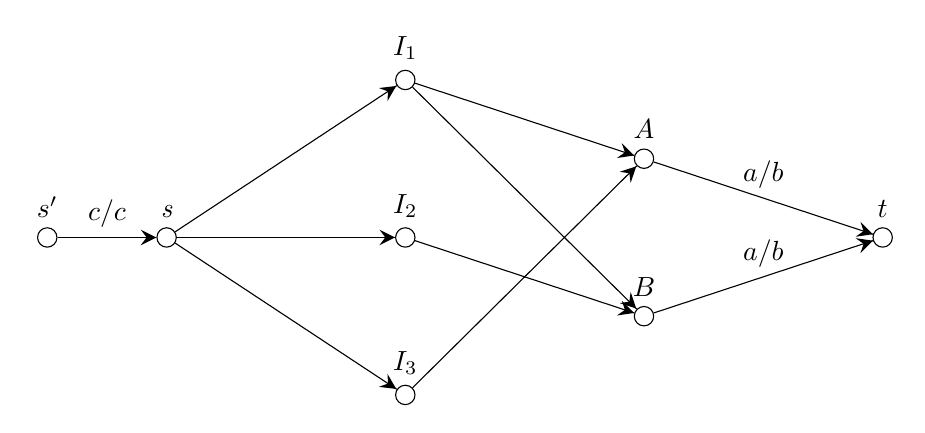
\begin{tikzpicture}[x=0.25\textwidth,
    every edge/.style={
        draw,
        postaction={decorate,
                    decoration={markings,mark=at position 1 with {\arrow[line width = 0.5mm]{stealth}}}
                   }
        }
]
\vertex (fonte') at (0,3) [label=above:$\textit{s}$] {};
\vertex (fonte) at (-0.5,3) [label=above:$s'$] {};
\vertex (I1) at (1,5) [label=above:$I_1$] {};
\vertex (I2) at (1,3) [label=above:$I_2$] {};
\vertex (I3) at (1,1) [label=above:$I_3$] {};
\vertex (A) at (2,4) [label=above:$A$] {};
\vertex (B) at (2,2) [label=above:$B$] {};
\vertex (dreno) at (3,3) [label=above:$t$] {};
\path
(fonte) edge node [above] {$c/c$} (fonte')
(fonte') edge (I1)
(fonte') edge (I2)
(fonte') edge (I3)
(I1) edge (A)
(I1) edge (B)
(I2) edge (B)
(I3) edge (A)
(A) edge node [above] {$a/b$} (dreno)
(B) edge node [above] {$a/b$} (dreno)
;
\end{tikzpicture}\]

A única diferença na construção do item b é que, ao invés de ligarmos
$s$ diretamente aos intervalos de monitoria, ligamos $s$ a cada dia da
semana i com demanda $d_i$ e capacidade $c$ e depois
criamos uma aresta com demanda 0 e capacidade 1 de
cada dia da semana para os intervalos que são naquele dia.

TODO: argumento que isso dá a solução certa

Abaixo está o mesmo exemplo do item a) com dias da semana. Para deixar
a visualização mais simples estamos colocando aqui apenas dois dias da
semana.

\[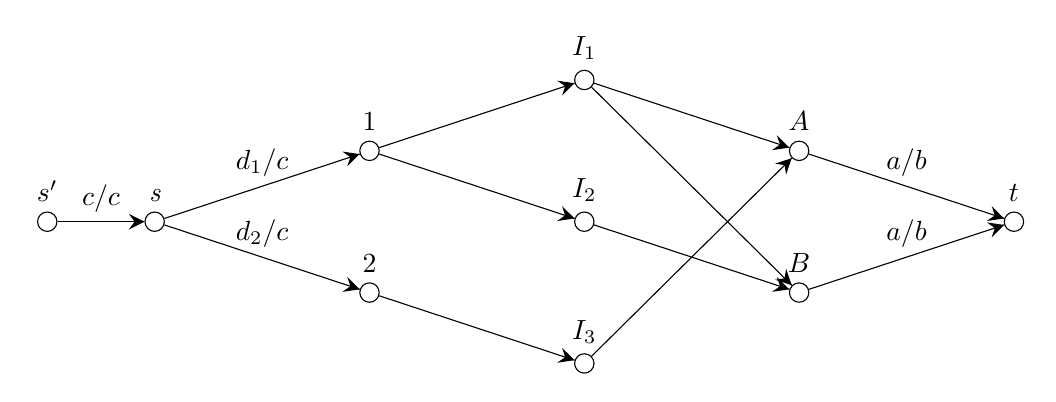
\begin{tikzpicture}[x=0.25\textwidth, scale=0.9,
    every edge/.style={
        draw,
        postaction={decorate,
                    decoration={markings,mark=at position 1 with {\arrow[line width = 0.5mm]{stealth}}}
                   }
        }
]
\vertex (fonte') at (0,3) [label=above:$\textit{s}$] {};
\vertex (fonte) at (-0.5,3) [label=above:$s'$] {};
\vertex (1) at (1, 4) [label=above:$1$] {};
\vertex (2) at (1, 2) [label=above:$2$] {};
\vertex (I1) at (2,5) [label=above:$I_1$] {};
\vertex (I2) at (2,3) [label=above:$I_2$] {};
\vertex (I3) at (2,1) [label=above:$I_3$] {};
\vertex (A) at (3,4) [label=above:$A$] {};
\vertex (B) at (3,2) [label=above:$B$] {};
\vertex (dreno) at (4,3) [label=above:$t$] {};
\path
(fonte) edge node [above] {$c/c$} (fonte')
(fonte') edge node [above] {$d_1/c$} (1)
(fonte') edge node [above] {$d_2/c$} (2)
(1) edge (I1)
(1) edge (I2)
(2) edge (I3)
(I1) edge (A)
(I1) edge (B)
(I2) edge (B)
(I3) edge (A)
(A) edge node [above] {$a/b$} (dreno)
(B) edge node [above] {$a/b$} (dreno)
;
\end{tikzpicture}\]

\subsubsection{Implementação}
\label{sec-3-3-3}

\begin{enumerate}
\item Fluxo máximo
\label{sec-3-3-3-1}

Vamos começar estudando o problema de encontrar o fluxo máximo de uma
rede $G$ em que $d_e = 0 \; \forall e \in E$ $f$. Vamos implementar aqui o
algoritmo de Ford-Fulkerson para resolver esse problema.

O algoritmo tem 2 partes:

\begin{enumerate}
\item Dado um caminho $P$ e partindo de um fluxo inicial $f$, obter um
novo fluxo $f'$ expandindo $f$ em $P$
\item Partindo do fluxo $f(e)$ = 0, expandir o fluxo enquanto for possível
\end{enumerate}


\begin{itemize}
\item Primeira parte:
\end{itemize}

O gargalo de um caminho é TODO: definir gargalo, explicar o código a seguir
Definimos aqui uma função que encontra o gargalo do caminho
\begin{minted}[]{python}
def encontra_gargalo(self, caminho):
    residuos = []
    for aresta in caminho:
        residuos.append(aresta.capacidade - self.fluxo[aresta])
    return min(residuos)
\end{minted}

Expandir o caminho é TODO: explicar o que é expandir o caminho,

\begin{minted}[]{python}
def expande_caminho(self, caminho):
    gargalo = self.encontra_gargalo(caminho)
    for aresta in caminho:
        self.fluxo[aresta] += gargalo
        self.fluxo[aresta.reversa] -= gargalo
\end{minted}

Com isso temos a parte 1 do algoritmo.

Para a parte 2, vamos precisar criar um fluxo $f$ com $f(e) = 0$ para
toda aresta $e$. Podemos fazer isso utilizando o seguinte método na
classe RedeDeFluxo():
\begin{minted}[]{python}
def cria_fluxo_inicial(self):
    for vertice, arestas in self.adj.iteritems():
        for aresta in arestas:
            fluxo[aresta] = 0
\end{minted}

TODO: explicar porque precisamos desse método e como ele funciona
Retorna um caminho de fonte a dreno passando pelos vértices
em caminho
\begin{minted}[]{python}
def encontra_caminho(self, fonte, dreno, caminho):
    if fonte == dreno:
        return caminho
    for aresta in self.encontra_arestas(fonte):
        residuo = aresta.capacidade - self.fluxo[aresta]
        if residuo > 0 and aresta not in caminho:
            resp = self.encontra_caminho(aresta.destino, dreno, caminho + [aresta])
            # TODO: explicar essa parte
            if resp != None:
                return resp
\end{minted}

Com todas as funções auxiliares prontas, podemos finalmente definir a
função que encontra o fluxo máximo.

TODO: explicar o algoritmo de fluxo máximo
\begin{minted}[]{python}
def fluxo_maximo(self, fonte, dreno):
    self.cria_fluxo_inicial()
    caminho = self.encontra_caminho(fonte, dreno, [])
    while caminho is not None:
        self.expande_caminho(caminho)
        caminho = self.encontra_caminho(fonte, dreno, [])
    return self.valor_do_fluxo(fonte)
\end{minted}

\item Fluxo válido com demandas não-nulas
\label{sec-3-3-3-2}

O nosso objetivo é encontrar um fluxo válido $f$ para uma rede $G =
(V, E)$ no caso em que as demandas são positivas.

Vamos construir uma rede $G' = (V', E')$ com um valor associado $d$
tal que $d_e = 0 \; \forall e \in E'$ de tal forma que um fluxo válido
para $G$ existe se e somente se o valor do fluxo máximo em $G'$ é
$d$. Em caso afirmativo, podemos construir um fluxo válido $f$ para
$G$ rapidamente a partir de qualquer fluxo máximo $f'$ de $G'$.

Construimos $G'$ da seguinte forma:

\begin{itemize}
\item Criamos um vértice em $G'$ para cada vértice $G$
\item Adicionamos uma fonte adicional $F$ e um dreno adicional $D$ a $G'$
\item Definimos o saldo de cada vértice $v \in V$ como: \[
  \textrm{saldo}(v) = \sum_{e \text{ saindo de }v}d_e - \sum_{e \text{
  chegando em }v}d_e \]
\item Se $\mathrm{saldo}(v) > 0$ adicionamos uma aresta $(v, D,
  \mathrm{saldo}(v), 0)$ a $G'$
\item Se $\mathrm{saldo}(v) < 0$ adicionamos uma aresta $(F, v,
  -\mathrm{saldo}(v), 0)$ a $G'$
\item Para cada aresta $e = (\mathrm{origem, destino, capacidade,
  demanda}) \in E$, crie uma aresta $e' = (\mathrm{origem, destino,
  capacidade - demanda, 0})$ em $G'$
\end{itemize}

Codificando a construção acima:
\begin{minted}[]{python}
def cria_rede_com_demandas_nulas(G):
    G_ = RedeDeFluxo()
    G_.novo_vertice('F')
    G_.novo_vertice('D')
    for vertice, arestas in G.adj.iteritems():
        G_.novo_vertice(vertice)
        saldo = sum(e.demanda for e in arestas)
        if saldo > 0:
            G_.nova_aresta(vertice, 'D', saldo,0)
        elif saldo < 0:
            G_.nova_aresta('F', vertice, -saldo, 0)
    for arestas in G.adj.values():
        for a in arestas:
             if not a.eh_reversa:
                 G_.nova_aresta(a.origem,
                                a.destino,
                                a.capacidade - a.demanda,
                                0)
\end{minted}
TODO: provar que soluções de um são também soluções do outro
\end{enumerate}


\subsubsection{Complexidade}
\label{sec-3-3-4}

\section{Exercício 4.5 (Tardos)}
\label{sec-4}

\subsection{Enunciado}
\label{sec-4-1}

Vamos considerar uma rua campestre longa e quieta, com casas
espalhadas bem esparsamente ao longo da mesma. (Podemos imaginar a
rua como um grande segmento de reta, com um extremo leste e um
extremo oeste.) Além disso, vamos assumir que, apesar do ambiente
bucólico, os residentes de todas essas casas são ávidos usuários de
telefonia celular.

Você quer colocar estações-base de celulares em certos pontos da
rodovia, de modo que toda casa esteja a no máximo quatro milhas de
uma das estações-base. Dê um algoritmo eficiente para alcançar esta
meta, usando o menor número possível de bases.


\section{Exercício 8.19 (Tardos)}
\label{sec-5}

\subsection{Enunciado}
\label{sec-5-1}

Um comboio de navios chega ao porto com um total de $n$ vasilhames
contendo tipos diferentes de materiais perigosos.
Na doca, estão $m$ caminhões, cada um com capacidade para até $k$
vasilhames.  Para cada um dos dois problemas, dê um algoritmo
polinomial ou prove NP-completude:


a) Cada vasilhame só pode ser carregado com segurança em alguns
   dos caminhões. Existe como estocar os $n$ vasilhames nos $m$
   caminhões de modo que nenhum caminhão esteja sobrecarregado, e
   todo vasilhame esteja num caminhão que o comporta com segurança?


b) Qualquer vasilhame pode ser colocado em qualquer caminhão,
   mas alguns pares de vasilhames não podem ficar juntos num mesmo
   caminhão. Existe como estocar os $n$ vasilhames nos $m$
   caminhões de modo que nenhum caminhão esteja sobrecarregado e
   que nenhum dos pares proibidos de vasilhames esteja no mesmo
   caminhão?
% Emacs 24.4.1 (Org mode 8.2.10)
\end{document}
